\documentclass{article}
\usepackage[utf8]{inputenc}
\usepackage{listings}
\usepackage{color}
\usepackage{tikz}
\usetikzlibrary{shapes}

\definecolor{dkgreen}{rgb}{0,0.6,0}
\definecolor{gray}{rgb}{0.5,0.5,0.5}
\definecolor{mauve}{rgb}{0.58,0,0.82}

\lstset{frame=tb,
  language=C,
  aboveskip=3mm,
  belowskip=3mm,
  showstringspaces=false,
  columns=flexible,
  basicstyle={\small\ttfamily},
  numbers=none,
  numberstyle=\tiny\color{gray},
  keywordstyle=\color{blue},
  commentstyle=\color{dkgreen},
  stringstyle=\color{mauve},
  breaklines=true,
  breakatwhitespace=true,
  tabsize=3
}

\begin{document}

\title{Relat\'orio Fase II}
\date{}

\maketitle

\begin{itemize}
    \item \textbf{Introdu\c c\~ao} \\
    Nesta fase do projeto devemos, utilizando o c\'odigo que interpreta c'odigo de cada rob\^o fornecido pelo usu\'ario, inserir novos comandos e criar estruturas para que a base do jogo esteja formada. Dentre elas est\~ao os tipos de \textbf{terreno}, o \textbf{Grid Hexagonal}, uma matriz onde o jogo se passar\'a, \textbf{chamadas de sistema}, onde o rob\^o pede ao sistema para realizar uma a\c c\~ao, \textbf{cria\c c\~ao e destrui\c c\~ao de ex\'ercitos} de rob\^os e um atualizador do jogo, ou \textbf{game loop}.
    
    \item \textbf{Arena} \\
    A Arena \'e onde o jogo ocorre. Sua implementa\c \~ao envolve uma \textit{struct} que cont\'em o Grid Hexagonal, representando o tabuleiro, um vetor que armazena os ex\'ercitos assim como dois inteiros, um representando a \'ultima posi\c c\~ao livre do vetor de ex\'ercitos e outro representando o tempo decorrido de jogo.
    \begin{lstlisting}
        // Arena
        typedef struct {
        	Grid grid;
        	int tempo;
        	Maquina*[100] exercitos;
        	int lastFree;
        } Arena;

    \end{lstlisting}
    \item \textbf{C\'elula} \\
    Uma C\'elula \'e uma struct da forma:
    \begin{lstlisting}
        // Celula
        typedef struct {
          Terreno t;
          Base b;
          Cristais c;
          Ocupacao o;
        } Celula;
    
    \end{lstlisting}
    Com esses dados, listamos o que cada c\'elula do Grid necessita para que o jogo funcione bem. Assim como \'e dedut\'ivel, o \textit{Terreno t} indica que tipo de terreno a c\'elula possui. A \textit{Base b} determina se a c\'elula configura uma base e se \'e amiga ou inimiga. \textit{Cristais c} \'e um inteiro que possui o n\'umero de cristais contidos na c\'elula. Por \'ultimo, a \textit{Ocupa\c \~ao o} diz se a c\'elula est\'a ocupada e se quem a ocupa \'e amigo ou inimigo.
    
    \item \textbf{Grid Hexagonal} \\
    O Grid Hexagonal \'e apenas uma matriz de c\'elulas onde o jogo ser\'a realizado. Ele est\'a definido da forma:
    \begin{lstlisting}
        typedef struct Celula** Grid;
    
    \end{lstlisting}
    Ele \'e inicializado da forma:
    \begin{lstlisting}
    arena->grid = malloc(nrows * sizeof(Grid *));
	for(int i = 0; i < nrows; i++) {
	    arena->grid[i] = malloc(ncolumns * sizeof(Grid));
	\end{lstlisting}
	
	Al\'em disso, por simplicidade e como poderemos mudar isso em fases futuras, inicializamos o tipo do terreno como o mesmo para toda c\'elula. Da mesma forma, elas come\c cam desocupadas e sem base com um n\'umero fixo de cristais.\\
	Optamos por utilizar o grid como na imagem abaixo:\\
	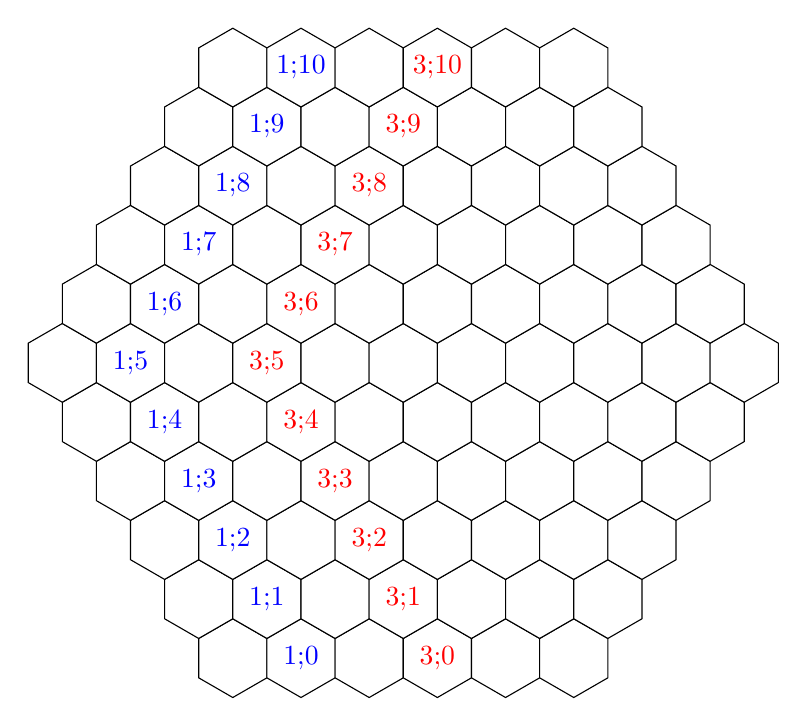
\begin{tikzpicture} [hexa/.style= {shape=regular polygon,regular polygon sides=6,minimum size=1cm, draw,inner sep=0,anchor=south,fill=white,rotate=30}]
    \foreach \j in {0,...,5}{%
        \pgfmathsetmacro\end{5+\j} 
        \foreach \i in {0,...,\end}{%
            \node[hexa] (h\i;\j) at ({(\i-\j/2)*sin(60)},{\j*0.75}) {};}  }      
    \foreach \j in {0,...,4}{%
        \pgfmathsetmacro\end{9-\j} 
        \foreach \i in {0,...,\end}{%
            \pgfmathtruncatemacro\k{\j+6}  
            \node[hexa] (h\i;\k) at ({(\i+\j/2-2)*sin(60)},{4.5+\j*0.75}) {};}  } 

  \foreach \k in {0,...,10}  {\node [circle,red,minimum size=1cm] at (h3;\k) {3;\k};} 
   \foreach \k in {0,...,10}  {\node [circle,blue,minimum size=1cm] at (h1;\k) {1;\k};}   
\end{tikzpicture}

    Isso facilitou a implementa\c cao de movimentos e o acesso \`as celulas vizinhas.
    \item \textbf{Game Loop} \\
    Esta \'e fun\c \~ao respons\'avel pela atualiza\c c\~ao do jogo do tempo $t$ para o tempo $t+1$:
    \begin{lstlisting}
    void atualiza(Arena *arena, int ciclos);
    
    \end{lstlisting}
    Nada mais que um \textit{loop} que percorre o vetor de rob\^os da Arena e executa as instru\c c\~oes fornecidas ao rob\^o um n\'umero \textit{ciclos} de vezes.\\
    Dessa forma, o \textit{game loop} \'e formado por uma s\'erie de chamadas desta fun\c c\~ao, utilizadas at\'e que um dos times saia vencedor.
    
    \item \textbf{System Calls} \\
    As chamadas de sistema s\~ao um conjunto de fun\c c\~oes que, dados \textit{a\c c\~ao} e \textit{dire\c c\~ao}, verifica se \'e uma a\c c\~ao v\'alida e executa no rob\^o que a pediu. Dentre as a\c c\~oes poss\'iveis est\~ao: \textit{mover, pegar, atacar, depositar}. Logo, o usu\'ario faz uma chamada da forma:
    \begin{lstlisting}
        SYS <ACTION> <DIRECTION>
    \end{lstlisting}
    Temos as a\c c\~oes:
    \begin{enumerate}
        \item MOVE
        \begin{lstlisting}
        void moveMachine(Arena *A, Maquina *m, Direction d);
        \end{lstlisting}
        Esta fun\c c\~ao apenas "olha" se a posi\c c\~ao correspondente a dire\c c\~ao \textit{d} est\'a ocupada e atualiza a posi\c c\~ao atual do rob\^o caso contr\'ario.
        
        \item GRAB
        \begin{lstlisting}
        void grabCrystal(Arena *A, Maquina *m, Direction d);
        \end{lstlisting}
        Esta fun\c c\~ao apenas verifica se a posi\c c\~ao correspondente a dire\c c\~ao \textit{d} possui cristais e diminui a quantidade de cristais da c\'elula em uma unidade, aumentando a do rob\^o na mesma propor\c c\~ao.
        
        \item DEPO
        \begin{lstlisting}
        void depositCrystal(Arena *A, Maquina *m, Direction d);
        \end{lstlisting}
        Esta fun\c c\~ao retira cristal do rob\^o e aumenta a da c\'elula, amos em uma unidade.
        \item ATTK
        \begin{lstlisting}
        void attackMachine(Arena *A, Maquina *m, Direction d);
        \end{lstlisting}
        Esta fun\c c\~ao apenas verifica se h\'a um rob\^o do time inimigo na posi\c c\~ao correspondente e, por enquanto, se houver, imprime uma mensagem na sa\'ida padr\~ao. Futuramente pretendemos implementar um sistema de pontos de vida nos rob\^os, al\'em de pontos de ataque e defesa para que esta fun\c c\~ao se mostre \'util.
    \end{enumerate}
    
    \item \textbf{O m\'etodo ATR} \\
    Assim como especificado, quando o usu\'ario chama ATR, a seguinte parcela de c\'odigo \'e executada:
    \begin{lstlisting}
        case ATR:
			tmp = desempilha(ip);
			empilha(tmp.arg, ip);
			break;
    \end{lstlisting}
    Ou seja, o elemento do topo da pilha \'e retirado e empilhamos o atributo de n\'umero arg do elemento.
    \item \textbf{Cria\c c\~ao e destrui\c \~ao de ex\'ercitos} \\
    Essas fun\c c\~oes s\~ao simples varreduras pelo vetor de rob\^os da arena. Para fins de simplifica\c c\~ao, limitamos a quantidade de rob\^os da arena em 100, o que explica as constantes nas fun\c c\~oes. No momento inserimos uma quantidade size de rob\^os de um determinado time.
    \begin{lstlisting}
void InsereExercito(Arena *arena, int size, INSTR *p, int time) {
	
	for(int i = arena->lastFree; i < 100; i++){
		Maquina robo;
		robo = cria_maquina(p);
		robo->t = time;
		arena->exercitos[i] = robo;
	}

	if(size > 100-arena->lastFree) printf("The Arena is full.\n"); 
}
    \end{lstlisting}
    
    Decidimos por destruir um grupo de rob\^os utilizando o time que ele pertence.
    \begin{lstlisting}
void RemoveExercito(Arena *arena,Time t) {
	for(int i = 99; i >=0; i--) {
		if(arena->exercitos[i] != NULL && arena->exercitos[i]->t == t) {
			arena->exercitos[i] = NULL;
		}
	}
	
}	
    \end{lstlisting}
    
    \item \textbf{Dificuldades} \\
    A maior dificuldade nesta fase foi com o tratamento de vari\'aveis de diferentes tipos. O usu\'ario poder manipular diferentes tipos nos fez ter de extender a struct OPERANDO, tal qual a cada instru\c c\~ao associamos um tipo e um valor. O OPERANDO teve de fazer papel de C\'elula, uma struct, mas tamb\'em de uma dire\c c\~ao, um enum. Codificar isso em C, uma linguagem sem orienta\c c\~ao a objetos, foi o maior desafio desta fase.
    
    \item \textbf{Testes} \\
    
    \item \textbf{Conclus\~oes} \\

\end{itemize}
\end{document}
